\documentclass{sigchi}

% Use this command to override the default ACM copyright statement (e.g. for preprints).
% Consult the conference website for the camera-ready copyright statement.

%% EXAMPLE BEGIN -- HOW TO OVERRIDE THE DEFAULT COPYRIGHT STRIP -- (July 22, 2013 - Paul Baumann)
\clubpenalty=10000 
\widowpenalty = 10000
%% EXAMPLE END -- HOW TO OVERRIDE THE DEFAULT COPYRIGHT STRIP -- (July 22, 2013 - Paul Baumann)
\toappear{CS262A Class Project}

% Arabic page numbers for submission.
% Remove this line to eliminate page numbers for the camera ready copy
% \pagenumbering{arabic}


% Load basic packages
\usepackage{balance}  % to better equalize the last page
\usepackage{graphics} % for EPS, load graphicx instead
\usepackage{times}    % comment if you want LaTeX's default font
\usepackage{url}      % llt: nicely formatted URLs
\usepackage{color}    % now you can define colors
\usepackage{array}
\newcolumntype{L}[1]{>{\raggedright\let\newline\\\arraybackslash\hspace{0pt}}m{#1}}
\newcolumntype{C}[1]{>{\centering\let\newline\\\arraybackslash\hspace{0pt}}m{#1}}
\newcolumntype{R}[1]{>{\raggedleft\let\newline\\\arraybackslash\hspace{0pt}}m{#1}}


% llt: Define a global style for URLs, rather that the default one
\makeatletter
\def\url@leostyle{%
  \@ifundefined{selectfont}{\def\UrlFont{\sf}}{\def\UrlFont{\small\bf\ttfamily}}}
\makeatother
\urlstyle{leo}


% To make various LaTeX processors do the right thing with page size.
\def\pprw{8.5in}
\def\pprh{11in}
\special{papersize=\pprw,\pprh}
\setlength{\paperwidth}{\pprw}
\setlength{\paperheight}{\pprh}
\setlength{\pdfpagewidth}{\pprw}
\setlength{\pdfpageheight}{\pprh}

% Make sure hyperref comes last of your loaded packages,
% to give it a fighting chance of not being over-written,
% since its job is to redefine many LaTeX commands.
\usepackage[pdftex]{hyperref}
\hypersetup{
pdftitle={SIGCHI Conference Proceedings Format},
pdfauthor={LaTeX},
pdfkeywords={SIGCHI, proceedings, archival format},
bookmarksnumbered,
pdfstartview={FitH},
colorlinks,
citecolor=black,
filecolor=black,
linkcolor=black,
urlcolor=black,
breaklinks=true,
}

% create a shortcut to typeset table headings
\newcommand\tabhead[1]{\small\textbf{#1}}

% End of preamble. Here it comes the document.
\begin{document}

\title{Performance analysis of joins in reactive queries}

\numberofauthors{2}
\author{
   \alignauthor Amy Pavel\\
    \affaddr{University of California, Berkeley}\\
    \email{amypavel@berkeley.edu}
   \alignauthor Mitar Milutinovic\\
    \affaddr{University of California, Berkeley}\\
    \email{mitar@berkeley.edu}
}

\maketitle

\begin{abstract}
Simple document-oriented databases like MongoDB forgo many traditional features of relational databases in favor of better performance. 
This means that applications often need to build additional features on top of the simple provided features. 
For example, applications often have to resolve relationships between stored documents. 
Recursive queries incurred by resolving relationships introduce delays. 
To mitigate such delays, we developed PeerDB, a modification to MongoDB. 
PeerDB optimizes for the common use case where the main document only requires a subset of fields from any related documents. 
PeerDB stores subsets of related fields as subdocuments of the main document. 
In theory, this modification should reduce existing recursive read delays as applications will no longer need to recursively query documents in many cases. 
However, we have not quantitatively evaluated PeerDB to find out whether it improves performance of MongoDB. In addition, there is no method for automatically selecting which fields to embed using PeerDB.

We contribute a comparison of read and write times between three system: PeerDB, MongoDB and PostgreSQL. 
In addition, we make each comparison with both low-level queries and high-level web applications. 
We find that although PeerDB contributes to faster reads than other systems under some conditions, this performance gain comes with trade-offs (e.g. write time and traffic). 
To help developers manage these trade-offs when choosing which fields to embed, we propose and evaluate a new algorithm for automatically selecting which fields to embed based on a given read and write workload. 
Our algorithm compares many possible configurations using a novel cost model to predict expected impact, then returns the lowest cost configuration.
We test our algorithm under different workloads and parameter settings.
\end{abstract}

\vspace{-0.08in}
\keywords{
	MongoDB, PeerDB, PostgreSQL, Document stores, Reactive queries
}

\vspace{-0.08in}

\section{Introduction}

In the traditional SQL world of relational databases you do joins between related documents every time you read them from the database.
This makes reading slower, your database management system is redoing the same computation of joins for every read, and also horizontal scaling of a database to many instances is harder because every read might potentially have to talk to other instances.

NoSQL databases like MongoDB remove relations between documents and leave it to users to resolve relations on their own.
This often means fetching one document, observing which other documents it references, and recursively fetching those as well.
For many-to-many relations this leads to potentially large number of queries.
Because each of those documents are stand-alone and static, it is relatively easy and quick for a database management system like MongoDB to find and return them.
Such an approach is quick and it scales horizontally easily, but the downside is the multiple round trips you have to do in your code to get all documents you are interested in.
In modern web applications where program logic is often running directly in the browser, accessing data through a web API, those round trips become even worse because those queries are coming over the Internet where latency is much higher.

\begin{figure}[t]
\centering
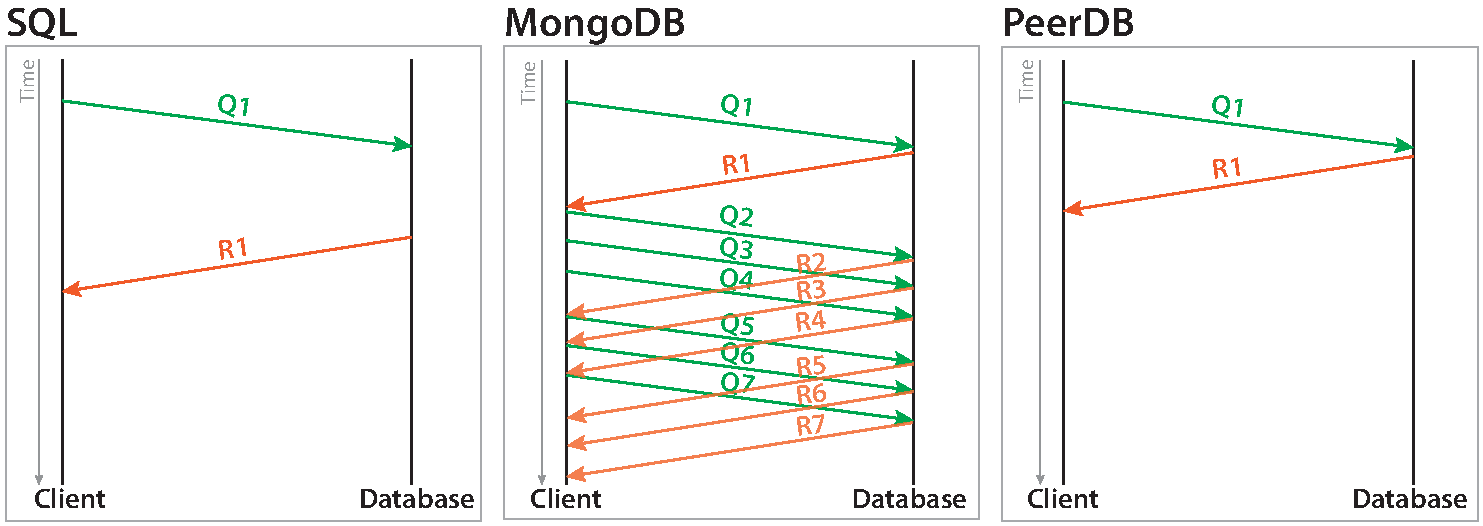
\includegraphics[width=0.9\columnwidth]{messages-many}
\caption{In traditional SQL, one query is needed to obtain data spawning multiple relations, but such results can be potentially large and time to compute joins is needed.
In MongoDB one has to create many subsequent queries to resolve relations, especially in many-to-many relations.
In PeerDB one has to simply fetch one document, with all relations already resolved, without any computation or communication among instances needed.}
\label{messages-many}
\end{figure}

Modern web frameworks like Meteor and DerbyJS introduced to the web developers community another family of database queries: reactive queries.
Using those frameworks you can make a database query where you receive results like you would for a normal query, but afterwards the query stays open and any changes to the results data is pushed to you in a reactive manner.
This allows you (or a framework you use) to respond to this changes in data.
For example, update a rendered template in a browser.
Programming in this way becomes much more declarative.

The downside is complexity a programer is faced with when making queries with joins.
While frameworks provide a simple to use primitive for making reactive queries against one MongoDB collection and receiving updates to documents in that collection as they are made for the open query, programming how manually resolved relations should respond to those updates in data is far from straightforward.
Community is slowly building libraries which are aiming to address these issues, but current solutions are made for specific type of queries and all share a common issue based on previously mentioned downside of manually resolving queries: high latency and number of queries.
As query results data is changed, queries for related documents have to be rerun again and again, even if the results of those new queries might not be different to previous ones, or even if only a smaller query for just a subset of documents would satisfy.

Thus, combination of joins in NoSQL databases with reactive queries pose a challenge to programers.
Luckily, we can observe that in many cases we are mostly interested only in few fields of a related document, again and again.
Instead of recomputing joins every time we read, we could use MongoDB's sub-documents feature to embed those fields along with the reference.
Instead of just storing the \verb|_id| of a related document, we could store also those few often used fields.
For example, if you are displaying blog posts, you want to display the author's name together with the blog post.
You will not really need only the blog post without the author name.
If an example blog post document looks like:

\begin{verbatim}
{
  "_id": "frqejWeGWjDTPMj7P",
  "body": "A simple blog post",
  "author": "yeK7R5Lws6MSeRQad",
  "tags": [
      "k7cgWtxQpPQ3gLgxa",
      "KMYNwr7TsZvEboXCw"
  ]
}
\end{verbatim}

Then the blog post with embedded common fields would look like:

\begin{verbatim}
{
  "_id": "frqejWeGWjDTPMj7P",
  "body": "A simple blog post",
  "author": {
    "_id": "yeK7R5Lws6MSeRQad",
    "name": "Wesley Crusher",
    "picture": "/img/yeK7R5Lws6MSeRQad.jpg"
  },
  "tags": [
    {
      "_id": "k7cgWtxQpPQ3gLgxa",
      "name": "announcement",
      "description": "Public announcements."
    },
    {
      "_id": "KMYNwr7TsZvEboXCw"
      "name": "test",
      "description": "Tests of the system."
    }
  ],
  "comments": [
    {
      "_id": "tMgj8mF2zF3gjCftS",
      "body": "A test comment."
    }
  ]
}
\end{verbatim}

Now we have to fetch only this one document and we have everything needed to display a blog post.
It is easy for us to query it and use it as any other document, with direct access to all subfields over which we can query as well.
For example, it is easy to query for all blog posts tagged with a given tag, provided that we have only its textual name to begin with.
We can make a MongoDB query \verb|{"tags.name": "test"}| to query all the documents tagged with tag \verb|test|.
The query can be reactive and we can easily get updates to it as data changes, without having to redo any queries for related documents.

Observe that blog post contains also comments data.
Each comment has a reference to a blog post of which a comment it is.
Information about a relation is thus stored in comment documents and not in posts themselves.
But we can embed this relation in the reverse direction as a list of subdocuments representing each comment referencing the blog post.

From the latency perspective such embedding of related documents makes queries much faster when reading.
Reactive queries do not have to requery related documents.
From the programmer's perspective this is much simpler to use because they can use familiar MongoDB queries directly.

Now, storing the author's name along with every blog post document brings an issue common when one is dealing with denormalized data.
What if user changes their name?
Then we have to update all those fields in documents referencing the user.
So we would have to make sure that anywhere in our code where we are changing the name, you are also updating fields in references.
What about changes to the database coming from outside of our code?

To address this issue and make easier for a programmer to embed subdocuments of related documents we designed and developer a layer on top of MongoDB called PeerDB.
Programmer can now in a declarative way specify relations between documents and which fields they would like to embed.
They have to define those references once and then PeerDB makes sure data stays in sync as it is changed across documents.
It does not matter where the changes come from, it will detect them and update fields in referenced sub-documents accordingly.
Instead of having to make recursive queries every time you read documents with related documents, PeerDB make those recursive queries once and store them into embedded documents.
The downside is that every modification to the data in the database triggers updates in documents in other collections.
While modifications to the document are stored quickly, changes have to propagate across all other documents.

To better understand performance characteristics of PeerDB we first present its implementation and then performance analysis approach and results.
We find that PeerDB performs better for reads than MongoDB alone and PostgreSQL for our benchmarks, when we manually select which fields to embed. 
Next, we present an algorithm to automatically pick which fields to embed based on expected impact of reads and writes under a user-specified workload. 
We find that our algorithm produces results that agree with intuition.
We conclude with our observations and discuss possible future work.


\section{Related Work}

Our algorithm embeds some document properties as sub documents in order to make it easier to reference whatever, our work is related to existing research in database cracking, materialized views, customizing key value stores, and discussions in the MongoDB development community.

\subsection{Materialized views}
A {\em view} is a function from a set of base tables to a derived table.
A {\em materialized view} is where you store tuples of a view in the database.
This way, database accesses to the materialized view can be faster than recomputing the view, especially when computing the view is expensive~\cite{Gupta1995}.
Materialized views for expensive queries would not work very well if you needed to recompute the materialized view whenever records were added or deleted, so past work has addressed how to efficiently maintain materialized views with incremental updates~\cite{Larson1985,Blakeley1986,Gupta1995,Zhou2007,Zhou2007a}.
Other work has provided methods for automatically selecting materialized views for a given workload in cases with lots of data~\cite{Agrawal2000,Yang1997}. 

Materialized views relate to our work because they create and update copies of data to decrease response time for expensive queries.
However, materialized views decrease database processing time on subsequent queries whereas we are interested in restructuring our data to decrease the number of round trips to the database. 

\subsection{Column store architecture and database cracking}
As we are restructuring our data to optimize read time, column store databases and database cracking are related to our project.
A {\em column store} relational database stores the values for each attribute contiguously, unlike traditional row store databases that store attributes of a record contiguously~\cite{Stonebraker}.
Such column store databases allow the DBMS to read only the values of the columns required for processing a given query so that they perform better in read-mostly applications.
Products such as Synbase IQ and KDB have demonstrated that this architecture improves performance~\cite{Stonebraker,French1995}. 

Idreos et al.~provide an optimization for column stores called {\em database cracking}~\cite{Pirk2007}.
In database cracking, a column $A$ is copied as $A_{CRK}$ when $A$ is first queried.
Then, $A_{CRK}$ is physically organized so that the values that satisfy the query are stored in contiguous space.
Thus, database cracking speeds up subsequent queries for similar values.
Follow up work proposed algorithms for updating cracked databases under high-volume insertions/deletions~\cite{Idreos2007}, and algorithms for increasing efficiency of tuple reconstruction for multi-attribute queries~\cite{Idreos2009}.

We are inspired by these successful methods for copying and reorganizing data to speed up read-heavy applications.
However, we can not directly use these methods in our case as they are intended for relational databases and we plan to reorganize data for fast reads on a non-relational database. 

\subsection{Adding functionality to non-relational databases} 
NoSQL-style databases sacrifice ``one-size-fits-all'' functionality for speed~\cite{Strauch}.
Thus, programmers build extra functionality on top of the simple database to satisfy application-specific needs.
Many research papers detail systems that supplement NoSQL databases to support complex quereies, ACID properties, and SLAs~\cite{Decandia2007,Chang,Beaver2010,Baker}. 

To our knowledge, no existing academic work addresses how to decrease the number of database round trips required to resolve recursive object relations in document store databases such as MongoDB.
The MongoDB manual~\cite{MongoDB2014} and a NoSQL survey paper~\cite{Strauch} notes application categories that inform when to (A) embed related objects and when to (B) reference related objects.
However, many applications do not comfortably fit either category.
So, application developers wrote guides for denormalizing objects so that you can both embed and reference objects~\cite{Wanschik2010}.
Unfortunately, following these guides requires a lot of effort and introduces opportunity for error.
Further, no one has qunatified benefits or downsides of denormalizing objects in MongoDB.

Our work creates and evaluates an application that supports denormalizing objects in MongoDB.



% \bibliography{papers}

\section{Automated embedded field selection}
PeerDB lets you embed fields to obtain faster reads on those fields at the expense of more time for writes and higher network traffic. 
For the benchmarks, we manually selected which fields to embed for the post document. 
Here we present a general algorithm for picking fields to embed in document based on the expected impact of embedding vs referencing a set of fields under a given workload.

\subsection{Overview}
Our algorithm optimizes the configuration of embedded fields in a main document $D$ according to a workload specification. 
For instance, if a post document $D$ references an author document, we could choose to embed all of the author's fields, none of the authors fields or some combination of these options. 
To choose between many possible configurations, our algorithm takes into account the expected field read and field write workloads specified by the user along with expected field size. 
Then, the algorithm assigns a cost to each configuration based on an approximate cost model. The algorithm returns the user the lowest cost configuration. 
The user uses this configuration to specify which fields to embed under their expected workload.

\subsection{Workload specification}
For queries to a given document, $D$, users need to supply how often they will query each all document fields and fields in related documents $D_R$. 
Specifically, for all fields $f_i \in D, D_R$ users specify, an expected frequency of reads originating from $D$ for each field, $E_R(f_i)$, an expected frequency of writes for each field, $E_W(f_i)$, and an expected size of each field $E_S(f_i)$. 

\subsection{Cost model}
Our cost model assigns a cost to a document configuration $C =$\{$c_1, c_2, ... c_n | c_i = 1 \text{ if field } f_i \in D_R \text{ is embedded }$\} considering expected read time, $R$, write time $W$, and traffic $T$ under a given workload specification, $S$.
$$Cost(C,S) = w_R*R + w_W*W + w_T*T$$ 
The parameters $w_R$ and $w_W$ allow the user to set the importance of the read-time and write-time respectively. 
For instance, the user may set the $w_R$ higher than $w_W$ in the case that website visitors read documents, but only admins write documents. 
As we do not consider the network traffic of calls other than those for the given document and it's fields, $w_T$ can be used to adjust the importance of keeping the number of messages passed as a result of document calls to a minimum.

\subsubsection{Computing read-time term, $R$}
The read-time term takes into account the read-times for all document fields and referenced document fields in a given configuration, $C$, for a given workload, $S$. 
$F$ means all fields $f_i$. 
We define $F_0$ as all fields $f_i$ where $c_i = 0$ and $F_1$ as all fields $f_i$ where $c_i = 1$. $F_D$ encompasses all fields in the base document which are not assigned in the configuration. 
The equation for $R$ also takes into account the time to request data, $M$, and the time to read one KB of data $K$:
\begin{align*}
R =& [M + max(E_R(f_i) \forall f_i \in F_1 \cup F_D)*\sum_{f_i \in F_1 \cup F_D} K*E_S(f_i)\\
& + \sum_{D_{R_i} \in D_R} \{M + max(E_R(f_i) \forall f_i \in D_{R_i} \cap F_0)\\
& * \sum_{f_i \in D_{R_i} \cap F_0} K*E_S(f_i)\} + P]
\end{align*}
The first summation calculates the expected read time for all document fields ($F_D$) and embedded fields ($F_1$). 
The second summation adds the expected read time for all secondary requests for referrenced documents and all time required to read the fields ($F_0$) of those documents. 
Because we assume we read all data from each document when we fetch it, the $max$ terms calculate how many times we need to fetch each document to match the required field reads. 
Overall, this equation shows that embedding a field saves read time for secondary requests incurred by referenced documents and their fields. 
We can see that embedding fields will decrease read-time in cases where the cost of a secondary request is high, or where the referenced documents are large.

Finally, $P$ is the penalty for inconsistency. 
If a read occurs before the write data is consistent, the read must recursively reference the referred document. 
$P$ accounts for the additional time for reacursively referencing the referred document as it was not covered in the other summations. 
For each embedded document, we add back on the time to retrieve the referenced document multiplied by the chance that the field is read while the data is in consistent, $I(f_i)$, which depends the frequency of writes and reads. 
Here $D_{R_{F_1}}$ refers to all documents that have an embedded field. 
$$P = I*\sum_{D_{R_i} \in D_{R_{F_1}}} [M+\sum_{f_i \in D_{R_i}} K*E_S(f_i)*E_R(f_i)]$$
In our implementation we set $I(f_i) = 0 \forall f_i \in F$. 
In future work, we will use detailed analysis to figure out how to relate the frequency of writes and reads to the chance that the read data is inconsistent. 
Like $M$ and $K$, this term will be unique to each system.

\subsubsection{Computing the write-time term $W$}
The write-time term takes into account the write times for all $f_i \in D, D_R$ for a given configuration $C$ and workload $S$. 
\begin{align*}
W =& [\sum_{f_i \in F_1} K*E_S(f_i)*E_W(f_i)\\
& + \sum_{f_i \in F} K*E_S(f_i)*E_W(f_i)]
\end{align*}
The first summation counts time for embedded fields, and the second summation counts time for all fields. This means embedded fields require two writes to update the referenced document whereas referenced documents only require one write. 
The write-time term $W$ displays that embedding fields will not be beneficial in write-heavy workloads.

\subsubsection{Computing the traffic term, $T$}
We add the term $T$ with its weight $w_T$ to allow the user to adjust how important it is to keep the network traffic from PeerDB low. 
$T$ is the number of messages passed based on reads and writes. 
\begin{align*}
T=& 2*|D\text{ reads}| + 2*|D_R\text{ reads}|\\
& + 4*|\text{embedded writes}| + 2*|\text{referenced writes}| 
\end{align*}

\subsection{Picking a configuration}
The total number of possible configurations for any schema is $2^n$ where $n$ represents the number of fields in referenced documents. 
In our implemnentation, $n$ is small so we use a brute force approach to find the configuration with the lowest cost. 
In cases where $n$ is large, we could apply a greedy algorithm or simulated annealing to find a near-optimal answer.

\subsection{Evaluation}
We implemented our model and tested it on one schema (Figure~\ref{fig:schema}) under several different workload specifications and parameter weightings. 

First, we ran our algorithm with the illustrated schema (Figure~\ref{fig:schema}) and workload specification (Table~\ref{workload}) with the parameter settings $w_R = 1, w_W = 0, w_T = 0$. Under these settings, the algorithm tells us that the lowest cost configuration embeds the author name and tag name, but no other fields. 
This is not surprising: only considering the read-time term, we expect fields often read with post that are not large to be embedded. 
The author picture field is large and only occasionally read with $D$.
As a result, the algorithm does not embed the author picture to avoid fetching it on every post query.

Setting the parameters to $w_R = 0, w_W = 1, w_T = 0$ (only considering writes), the algorithm tells us to not embed any fields, because every embedded field incurs extra write time.
Finally, setting the parameters to only pay attention to the messages passed, $w_R = 0, w_W = 0, w_T = 1$ we get that we should embed all fields except author bio and tag description. 
The algorithm picks this configuration because we provided a read-heavy workload, and each non-embedded field requires extra messages to read. 

For this schema and workload, if we set the parameters to $w_R = 1, w_W = 1, w_T = 0$ we unsurprisingly get the same configuration as suggested by considering the read time alone. 
However, if we switch the expected read values in the workload specification with the expected write values in the specification and leave the parameters as  $w_R = 1, w_W = 1, w_T = 0$, the algorithm tells us to not embed any fields. 

Overall, our algorithm agrees with intuition in these cases. Such an algorithm can pick the lowest cost fields to embed based on a schema and an expected workload specification.

\subsection{Implementation}
This algorithm was implemented in unoptimized Python code on a MacBook Pro. Each run of the algorithm to consider all embeddings and return the lowest cost configuration took around ~2ms.

\begin{figure}[t]
\centering
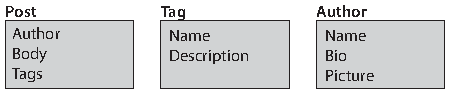
\includegraphics[width=3.33in]{figures/algorithm-schema.pdf}
\caption{We tested our algorithm with a schema where post was the main document $D$, and the post referenced related documents author and tags. All possible configurations of post are embedding all related document fields, none of the related document fields, or any combinations of the related document fields.}
\label{fig:schema}
\end{figure}


\begin{table}
  \small
  \begin{center}
  \begin{tabular}{|l|l|l|l|}
    %\hline
    \hline
    Field & $E_S$ (KB) & $E_R$ (reads/day) & $E_W$ (writes/day)\\ \hline
    Author name & .1 & 1000 & 1 \\
    Author bio & 1 & 0 & 5 \\ 
    Author picture & 1000 & 50 & 5 \\ 
    Tag name & .1 & 1000 & 1 \\ 
    Tag description & 1 & 0 & 2 \\ 
    Post body & 10 & 1000 & 1 \\ \hline

  \end{tabular}
  \end{center}
  \caption{Here is a sample workload specification for our schema. We quantify expected reads and writes per day over fields from all post documents. In this case, we have a read-heavy workload where most views include the author name, post body, and tag names with the post, but only some views include the author picture.}
  \label{workload}
  \vspace{-4mm}
\end{table}

In future work we will rigorously test our model to make sure it matches the benchmark expectations. 

\subsection{Discussion}
Although useful for many applications, our model makes several simplifications. 
For instance, our model does not take into account the reverse field feature of PeerDB. 
Further, our model does not take into account the possibility of embedding an entire referenced document instead of using PeerDB. 
Embedding without PeerDB the document instead of providing a reference is helpful in cases where you only reference the embedded document from the parent document~\cite{MongoDB2014}. 
In the future, we will add this option by augmenting the model and workload specification to include querying documents aside from the main document $D$. 
Our model also assumes that you read all information in a document when you fetch it. 
In the future we could let the user specify which combinations of fields they would read and adjust our cost model to handle such specifications.

We also made other minor simplifications, such as using the same constants $K$ and $M$ for all writes and reads. 
In reality, these numbers are different for writes and reads. 
In the future, we could provide an application to learn these constants for any given system. 


\section{PeerDB implementation}

PeerDB is implemented as a library for Meteor web framework.
It provides a declarative way to define database schema for documents and relations between document for your Meteor web application.
Together with specifying relations, you can also specify which fields should be embedded as subdocuments for both forward and backwards relations.
Currently, PeerDB requires programmer to decide if and which fields to embed.
That decision can often be made on program's logic and profiling of queries, in a similar way one would be deciding about existence of an index on a field.
Both embedding and indexes make a trade-off between faster read times on an expense of write times.

Additionally, PeerDB provides an easy way to define generator fields (fields which value is computed based on values of other fields) and generic triggers.

It uses an abstraction over MongoDB oplog to implement all above mentioned features.
MongoDB oplog originally serves for replication among multiple MongoDB instances, sending a stream of all changes from master to slaves.
We can connect to this same oplog to observe all changes in the database and determine if a change is connected to a field which is embedded in a related document.
If this is so, PeerDB issues update queries which update all those fields in subdocuments in related documents.

As currently implemented, PeerDB issues updates queries in a straightforward way, without any optimizations which might reduce the number of unnecessary updates queries.
Currently queries are issued and are left to MongoDB to determine that a particular query does not have anything to update.

PeerDB runs as a background process inside Meteor application, observing changes in the database and issuing the updates.
To scale, it provides a way to run as multiple separate processes/instances to distribute the load, each instance observing and reacting to just a subset of all documents based on their ID.

It is implemented in CoffeeScript and available as open source library at \url{https://github.com/peerlibrary/meteor-peerdb}.

\section{Performance analysis}

In this section we present the performance analysis and comparison of PeerDB-enabled queries vs. traditional approaches using relational DBMS and NoSQL database.

\subsection{Setup}

We approached the performance analysis by designing a simple data schema which consist of a one-to-many relation, many-to-many relation, and a reverse relation.
To easier understand it and discuss it, we assign to entities in the schema meaningful names of a simple blog application.
Figure \ref{schema} shows the entities and relations between them.

\begin{figure}[!h]
\centering
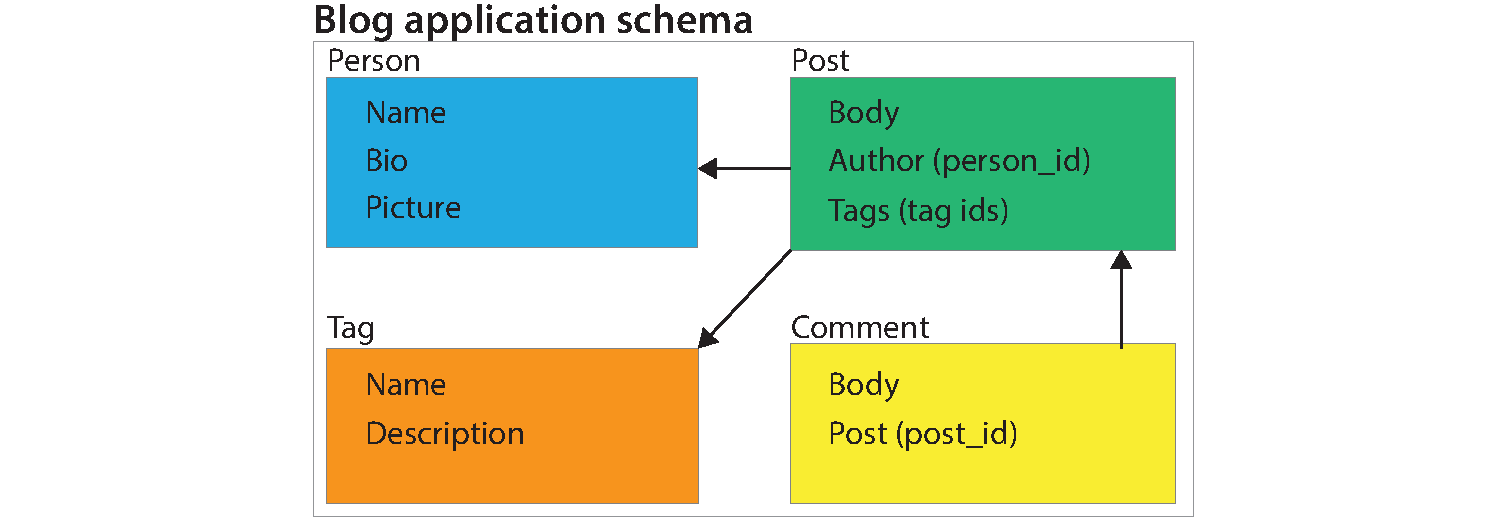
\includegraphics[width=0.9\columnwidth]{schema}
\caption{A blog post is the main entity we are querying. It has one-to-many \emph{author} relation to person entity and many-to-many \emph{tags} relation to tag entity. Comment entity has a one-to-many \emph{post} relation to the post entity, for which this relation is a reverse relation where we are interested in all comments made for a given post.}
\label{schema}
\end{figure}

To measure performance we decided to use a query which uses all relatons in the schema.
By querying for a blog post document, in addition to the post data itself, we want to get:
\begin{itemize}
\item name and picture of the author
\item name and description of all tags of the blog post
\item body of all blog post's comments
\end{itemize}

The concrete query we used is as follows: based on a string tag name, obtain all blog posts which are tagged with that tag, and for each blog post above mentioned additional data have to be available.

To be able to compare the measurements we implemented this schema and query in multiple systems:
\begin{itemize}
\item using PostgreSQL relational DBMS with low-level queries in Python
\item using PostgreSQL relational DBMS with high-level queries in Django, a Python based web framework
\item using MongoDB with low-level queries in Python
\item using MongoDB with high-level queries in Meteor
\item using MongoDB with PeerDB in Meteor
\item using MongoDB with PeerDB in Python
\end{itemize}

The motivation was to measure both low-level and high-level database interfaces to be able to compare difference between using a high-level web framework and not. To measure both traditional relational DBMS and NoSQL one. And of course to see how it works when using PeerDB and when not.

\begin{table}
  \small
  \begin{center}
  \begin{tabular}{|l|l|l|l|}
    %\hline
    \hline
    Entity & Number of documents\\
    \hline
    Person & 100 \\
    Tags & 100 \\ 
    Posts & 1000 \\ 
    Comments & 10000 \\ 
    \hline

  \end{tabular}
  \end{center}
  \caption{Basic number of documents used in the benchmark.}
  \label{numbers}
\end{table}

\begin{table}
  \small
  \begin{center}
  \begin{tabular}{|l|l|l|l|}
    %\hline
    \hline
    Field & Size in bytes\\
    \hline
    Person name & 11 \\
    Person bio & 1000 \\ 
    \emph{Person picture} & 10 \\
    Tag name & 11 \\ 
    \emph{Tag description} & 10 \\
    Post body & 1000 \\
    \emph{Comment body} & 10 \\
    \hline

  \end{tabular}
  \end{center}
  \caption{Basic size of fields in documents used in the benchmark.
  \emph{Emphasized} are fields which we varied in size.}
  \label{sizes}
\end{table}

Basic number of documents used in the benchmark are shown in table \ref{numbers}, and basic size of fields in documents used in the benchmark in table \ref{sizes}.
Basic number of tags per post was 10.
We uniformly distributed all comments across all blog posts. For future work we could consider using a long-tailed distribution.

We scaled this basic numbers and sizes to vary:
\begin{itemize}
\item number of documents, we used multiplication factors 1, 2, 4, 6, 8, 10
\item size of person picture, tag description, and comment body fields in documents, we used sizes 10, 100, 1000, 10000, 100000
\end{itemize}

When varying one dimension we kept the other at its basic value.

In addition, for two PeerDB based systems (Meteor and Python) we additionally vary how many PeerDB instances are observing and handling the changes in the database, running all above variations on 1, 2, 4, 6, 8 and 10 instances.

\subsection{Execution}

For execution of the benchmark we prepared a Docker image with Ubuntu 14.04.1 Linux as the base system, and PostgreSQL 9.3.5 and MongoDB 2.4.9.
We run that image on three Linux based 64bit systems, each with 32 GB of memory and 2 Intel Xeon X5670 2.93GHz processors with 6 cores each processor.
We varied the type of a running program and parameters when running an image to obtain the following measurements.

\subsection{Results}

\begin{figure}%
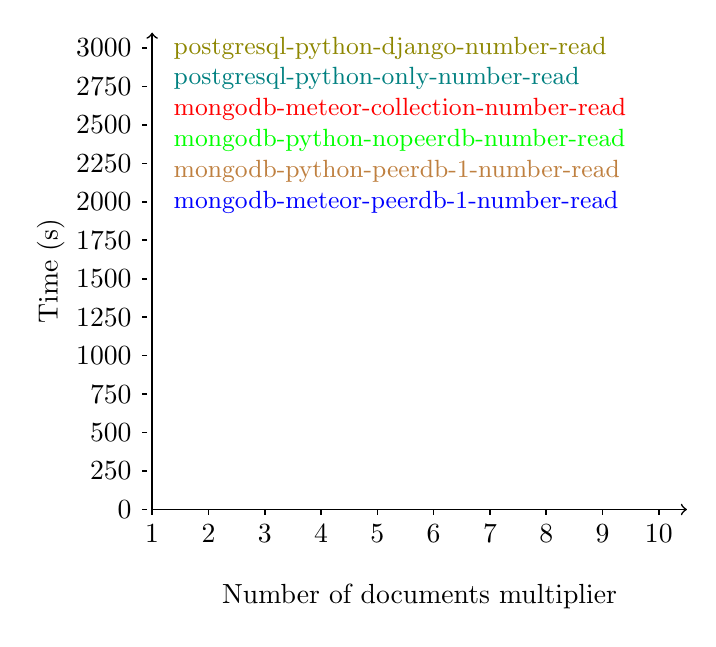
\begin{tikzpicture}[
	y=.003cm,
	x=1.1cm,
	semithick,
	scale=0.65
]

\draw[color=olive,thick] node[anchor=west] at (1.2,3000) {\small postgresql-python-django-number-read};
\draw[color=teal,thick] node[anchor=west] at (1.2,2800) {\small postgresql-python-only-number-read};
\draw[color=red,thick] node[anchor=west] at (1.2,2600) {\small mongodb-meteor-collection-number-read};
\draw[color=green,thick] node[anchor=west] at (1.2,2400) {\small mongodb-python-nopeerdb-number-read};
\draw[color=brown,thick] node[anchor=west] at (1.2,2200) {\small mongodb-python-peerdb-1-number-read};
\draw[color=blue,thick] node[anchor=west] at (1.2,2000) {\small mongodb-meteor-peerdb-1-number-read};

\draw[->] (1,0) -- coordinate (x axis) (10.5,0);
\draw[->] (1,0) -- coordinate (y axis) (1,3100);
\foreach \x in {1,...,10}
	\draw (\x,0pt) -- (\x,-3pt) node[anchor=north] {$\x$};
\foreach \y in {0,250,...,3000}
	\draw[xshift=1cm] (0pt,\y) -- (-3pt,\y) node[anchor=east] {$\y$};
\node[below=1.2cm,anchor=base] at (x axis) {Number of documents multiplier};
\node[left=1.2cm,rotate=90,anchor=base] at (y axis) {Time (s)};

\draw[color=red,thick] plot[mark=x,smooth] file {mongodb-meteor-collection-number-read.txt};
\draw[color=blue,thick] plot[mark=x,smooth] file {mongodb-meteor-peerdb-1-number-read.txt};
\draw[color=green,thick] plot[mark=x,smooth] file {mongodb-python-nopeerdb-number-read.txt};
\draw[color=brown,thick] plot[mark=x,smooth] file {mongodb-python-peerdb-1-number-read.txt};
\draw[color=olive,thick] plot[mark=x,smooth] file {postgresql-python-django-number-read.txt};
\draw[color=teal,thick] plot[mark=x,smooth] file {postgresql-python-only-number-read.txt};

\end{tikzpicture}%
\caption{number-read}%
\label{number-read}%
\end{figure}

\begin{figure}%
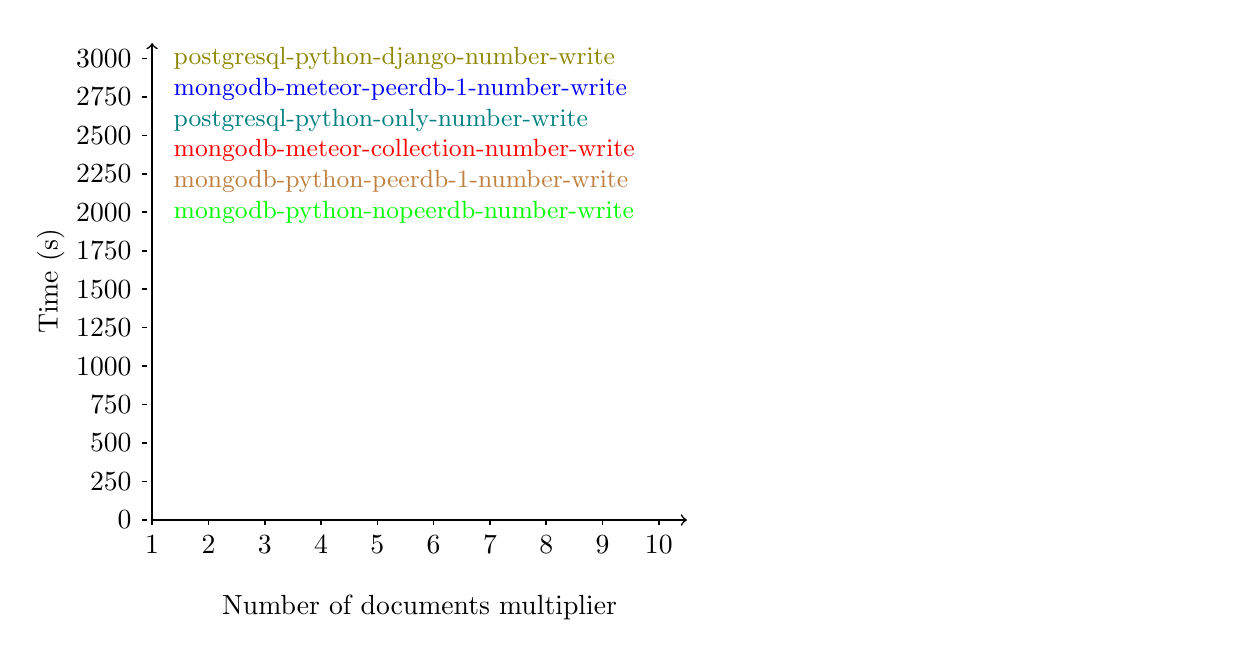
\begin{tikzpicture}[
	y=.003cm,
	x=1.1cm,
	semithick,
	scale=0.65
]

\draw[color=olive,thick] node[anchor=west] at (1.2,3000) {\small postgresql-python-django-number-write};
\draw[color=blue,thick] node[anchor=west] at (1.2,2800) {\small mongodb-meteor-peerdb-1-number-write};
\draw[color=teal,thick] node[anchor=west] at (1.2,2600) {\small postgresql-python-only-number-write};
\draw[color=red,thick] node[anchor=west] at (1.2,2400) {\small mongodb-meteor-collection-number-write};
\draw[color=brown,thick] node[anchor=west] at (1.2,2200) {\small mongodb-python-peerdb-1-number-write};
\draw[color=green,thick] node[anchor=west] at (1.2,2000) {\small mongodb-python-nopeerdb-number-write};

\draw[->] (1,0) -- coordinate (x axis) (10.5,0);
\draw[->] (1,0) -- coordinate (y axis) (1,3100);
\foreach \x in {1,...,10}
	\draw (\x,0pt) -- (\x,-3pt) node[anchor=north] {$\x$};
\foreach \y in {0,250,...,3000}
	\draw[xshift=1cm] (0pt,\y) -- (-3pt,\y) node[anchor=east] {$\y$};
\node[below=1.2cm,anchor=base] at (x axis) {Number of documents multiplier};
\node[left=1.2cm,rotate=90,anchor=base] at (y axis) {Time (s)};

\clip (-1,-100) rectangle (20,3200);

\draw[color=red,thick] plot[mark=x,smooth] file {mongodb-meteor-collection-number-write.txt};
\draw[color=blue,thick] plot[mark=x,smooth] file {mongodb-meteor-peerdb-1-number-write.txt};
\draw[color=green,thick] plot[mark=x,smooth] file {mongodb-python-nopeerdb-number-write.txt};
\draw[color=brown,thick] plot[mark=x,smooth] file {mongodb-python-peerdb-1-number-write.txt};
\draw[color=olive,thick] plot[mark=x,smooth] file {postgresql-python-django-number-write.txt};
\draw[color=teal,thick] plot[mark=x,smooth] file {postgresql-python-only-number-write.txt};

\end{tikzpicture}%
\caption{number-write}%
\label{number-write}%
\end{figure}

\begin{figure}%
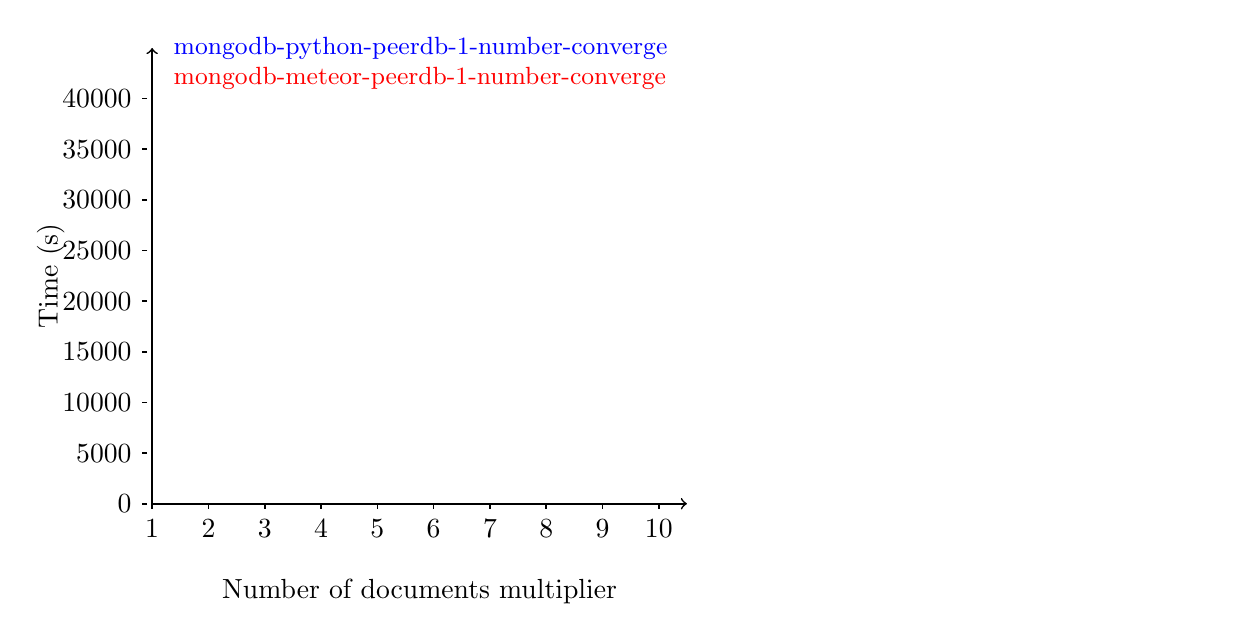
\begin{tikzpicture}[
	y=.0002cm,
	x=1.1cm,
	semithick,
	scale=0.65
]

\draw[color=blue,thick] node[anchor=west] at (1.2,45000) {\small mongodb-python-peerdb-1-number-converge};
\draw[color=red,thick] node[anchor=west] at (1.2,42000) {\small mongodb-meteor-peerdb-1-number-converge};

\draw[->] (1,0) -- coordinate (x axis) (10.5,0);
\draw[->] (1,0) -- coordinate (y axis) (1,45000);
\foreach \x in {1,...,10}
	\draw (\x,0pt) -- (\x,-3pt) node[anchor=north] {$\x$};
\draw[xshift=1cm] (0pt,0) -- (-3pt,0) node[anchor=east] {$0$};
\draw[xshift=1cm] (0pt,5000) -- (-3pt,5000) node[anchor=east] {$5000$};
\draw[xshift=1cm] (0pt,10000) -- (-3pt,10000) node[anchor=east] {$10000$};
\draw[xshift=1cm] (0pt,15000) -- (-3pt,15000) node[anchor=east] {$15000$};
\draw[xshift=1cm] (0pt,20000) -- (-3pt,20000) node[anchor=east] {$20000$};
\draw[xshift=1cm] (0pt,25000) -- (-3pt,25000) node[anchor=east] {$25000$};
\draw[xshift=1cm] (0pt,30000) -- (-3pt,30000) node[anchor=east] {$30000$};
\draw[xshift=1cm] (0pt,35000) -- (-3pt,35000) node[anchor=east] {$35000$};
\draw[xshift=1cm] (0pt,40000) -- (-3pt,40000) node[anchor=east] {$40000$};
\node[below=1.2cm,anchor=base] at (x axis) {Number of documents multiplier};
\node[left=1.2cm,rotate=90,anchor=base] at (y axis) {Time (s)};

\clip (-1,-100) rectangle (20,46000);

\draw[color=red,thick] plot[mark=x,smooth] file {mongodb-meteor-peerdb-1-number-converge.txt};
\draw[color=blue,thick] plot[mark=x,smooth] file {mongodb-python-peerdb-1-number-converge.txt};

\end{tikzpicture}%
\caption{number-converge}%
\label{number-converge}%
\end{figure}

\begin{figure}%
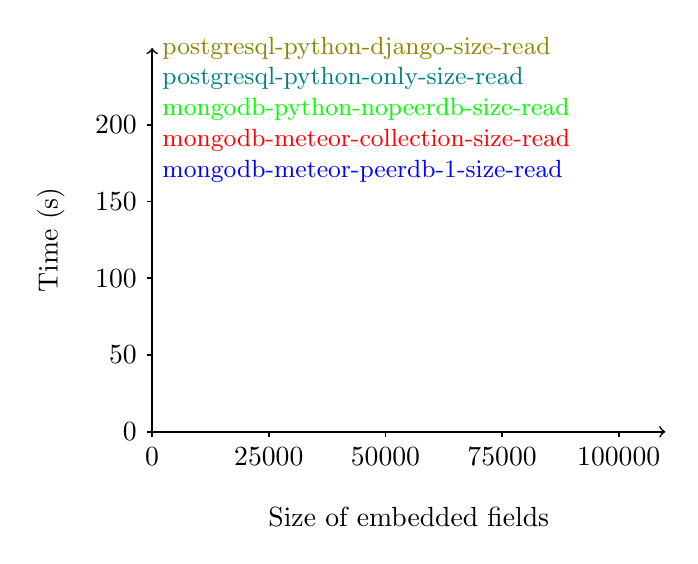
\begin{tikzpicture}[
	y=.03cm,
	x=0.00009cm,
	semithick,
	scale=0.65
]

\draw[color=olive,thick] node[anchor=west] at (1.2,250) {\small postgresql-python-django-size-read};
\draw[color=teal,thick] node[anchor=west] at (1.2,230) {\small postgresql-python-only-size-read};
\draw[color=green,thick] node[anchor=west] at (1.2,210) {\small mongodb-python-nopeerdb-size-read};
\draw[color=red,thick] node[anchor=west] at (1.2,190) {\small mongodb-meteor-collection-size-read};
\draw[color=blue,thick] node[anchor=west] at (1.2,170) {\small mongodb-meteor-peerdb-1-size-read};
%\draw[color=brown,thick] node[anchor=west] at (1.2,2200) {\small mongodb-python-peerdb-1-size-read};

\draw[->] (1,0) -- coordinate (x axis) (110000,0);
\draw[->] (1,0) -- coordinate (y axis) (1,250);
\foreach \x in {0,25000,50000,75000,100000}
	\draw (\x,0pt) -- (\x,-3pt) node[anchor=north] {$\x$};
\foreach \y in {0,50,...,200}
	\draw[xshift=0cm] (0pt,\y) -- (-3pt,\y) node[anchor=east] {$\y$};
\node[below=1.2cm,anchor=base] at (x axis) {Size of embedded fields};
\node[left=1.2cm,rotate=90,anchor=base] at (y axis) {Time (s)};

\draw[color=red,thick] plot[mark=x,smooth] file {mongodb-meteor-collection-size-read.txt};
\draw[color=blue,thick] plot[mark=x,smooth] file {mongodb-meteor-peerdb-1-size-read.txt};
\draw[color=green,thick] plot[mark=x,smooth] file {mongodb-python-nopeerdb-size-read.txt};
%\draw[color=brown,thick] plot[mark=x,smooth] file {mongodb-python-peerdb-1-size-read.txt};
\draw[color=olive,thick] plot[mark=x,smooth] file {postgresql-python-django-size-read.txt};
\draw[color=teal,thick] plot[mark=x,smooth] file {postgresql-python-only-size-read.txt};

\end{tikzpicture}%
\caption{size-read}%
\label{size-read}%
\end{figure}

\begin{figure}%
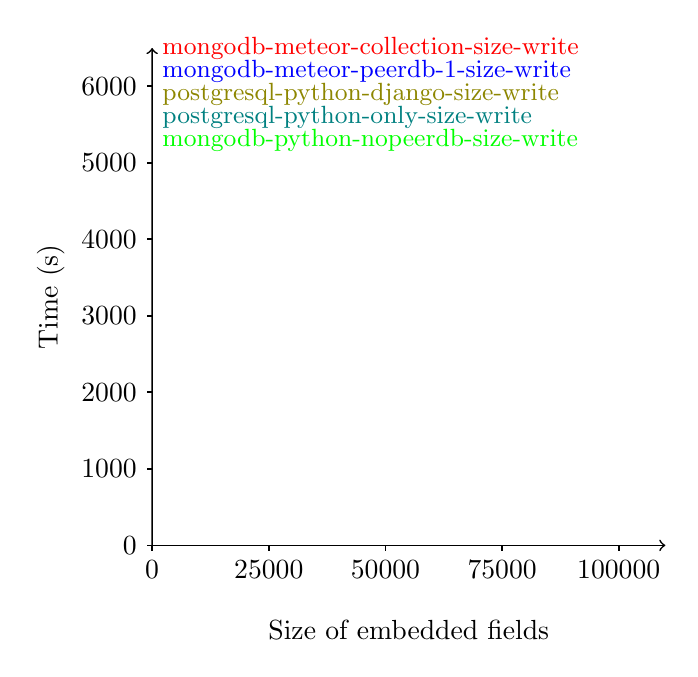
\begin{tikzpicture}[
	y=.0015cm,
	x=0.00009cm,
	semithick,
	scale=0.65
]

\draw[color=red,thick] node[anchor=west] at (1.2,6500) {\small mongodb-meteor-collection-size-write};
\draw[color=blue,thick] node[anchor=west] at (1.2,6200) {\small mongodb-meteor-peerdb-1-size-write};
\draw[color=olive,thick] node[anchor=west] at (1.2,5900) {\small postgresql-python-django-size-write};
\draw[color=teal,thick] node[anchor=west] at (1.2,5600) {\small postgresql-python-only-size-write};
\draw[color=green,thick] node[anchor=west] at (1.2,5300) {\small mongodb-python-nopeerdb-size-write};
%\draw[color=brown,thick] node[anchor=west] at (1.2,2200) {\small mongodb-python-peerdb-1-size-write};

\draw[->] (1,0) -- coordinate (x axis) (110000,0);
\draw[->] (1,0) -- coordinate (y axis) (0,6500);
\foreach \x in {0,25000,50000,75000,100000}
	\draw (\x,0pt) -- (\x,-3pt) node[anchor=north] {$\x$};
\foreach \y in {0,1000,...,6500}
	\draw[xshift=0cm] (0pt,\y) -- (-3pt,\y) node[anchor=east] {$\y$};
\node[below=1.2cm,anchor=base] at (x axis) {Size of embedded fields};
\node[left=1.2cm,rotate=90,anchor=base] at (y axis) {Time (s)};

\draw[color=red,thick] plot[mark=x,smooth] file {mongodb-meteor-collection-size-write.txt};
\draw[color=blue,thick] plot[mark=x,smooth] file {mongodb-meteor-peerdb-1-size-write.txt};
\draw[color=green,thick] plot[mark=x,smooth] file {mongodb-python-nopeerdb-size-write.txt};
%\draw[color=brown,thick] plot[mark=x,smooth] file {mongodb-python-peerdb-1-size-write.txt};
\draw[color=olive,thick] plot[mark=x,smooth] file {postgresql-python-django-size-write.txt};
\draw[color=teal,thick] plot[mark=x,smooth] file {postgresql-python-only-size-write.txt};

\end{tikzpicture}%
\caption{size-write}%
\label{size-write}%
\end{figure}

\begin{figure}%
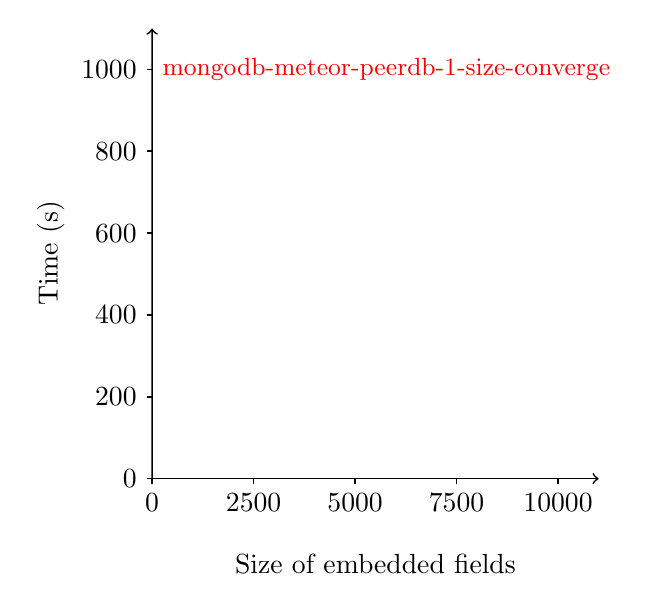
\begin{tikzpicture}[
	y=.008cm,
	x=.0008cm,
	semithick,
	scale=0.65
]

\draw[color=red,thick] node[anchor=west] at (1.2,1000) {\small mongodb-meteor-peerdb-1-size-converge};
%\draw[color=blue,thick] node[anchor=west] at (1.2,900) {\small mongodb-python-peerdb-1-size-converge};

\draw[->] (1,0) -- coordinate (x axis) (11000,0);
\draw[->] (1,0) -- coordinate (y axis) (0,1100);
\foreach \x in {0,2500,...,11000}
	\draw (\x,0pt) -- (\x,-3pt) node[anchor=north] {$\x$};
\foreach \y in {0,200,...,1000}
	\draw[xshift=0cm] (0pt,\y) -- (-3pt,\y) node[anchor=east] {$\y$};
\node[below=1.2cm,anchor=base] at (x axis) {Size of embedded fields};
\node[left=1.2cm,rotate=90,anchor=base] at (y axis) {Time (s)};

\draw[color=red,thick] plot[mark=x,smooth] file {mongodb-meteor-peerdb-1-size-converge.txt};
%\draw[color=blue,thick] plot[mark=x,smooth] file {mongodb-python-peerdb-1-size-converge.txt};

\end{tikzpicture}%
\caption{size-converge}%
\label{size-converge}%
\end{figure}



\section{automatic algorithm}

Automatic algorithm: Description (1 page)
Automatic algorithm: Experimental setup + Results (1/2 page)
Automatic algorithm: Discussion (1/2 page)


\section{Conclusions}

\section{Future work}
Our work leads to three main directions for future work: improvements of PeerDB, additional benchmarking, improvements to the automatic embedding algorithm and evaluation.
This section will address each of these future work areas in turn.

\subsection{Improving PeerDB}

\subsection{Benchmarking}

\subsection{Automatic algorithm}
One direction for improving the automatic algorithm is extending it's applicability to more use cases. For instance, the algorithm does not currently consider all possible sets of queries (only those that strictly augment the smallest set). In future work, we extend the model to encompass more query sets. As mentioned before, future work may also extend the algorithm to handle cases where we embed entire subdocuments without having the document separately referenced (no help from PeerDB). In addition, we want to extend it to handle reverse queries. Lastly, we will augment the automatic algorithm with a more global view of the workload and system so that we could jointly figure out embeddings for all documents at one time.

Another direction for improving the automatic algorithm is verifying and enhancing the accuracy of the cost model and input parameters. 
Future work could learn parameters, simulate possible configurations for greater accuracy, and compare our current cost model closely to actual system performance. 
We could also evaluate low cost configurations using our benchmarking system against high cost configurations to see if relative performance for these configurations confirms intuition.

One final direction for improving the automatic algorithm is assuring that it works at scale. Currently, our algorithm uses brute force to calculate the lowest cost embeddings. In cases where there are more possible combinations of embeddings we could use an existing optimization technique to find an approximate configuration. For instance, we could apply simulated annealing or a greedy approach.



% Balancing columns in a ref list is a bit of a pain because you
% either use a hack like flushend or balance, or manually insert
% a column break.  http://www.tex.ac.uk/cgi-bin/texfaq2html?label=balance
% multicols doesn't work because we're already in two-column mode,
% and flushend isn't awesome, so I choose balance.  See this
% for more info: http://cs.brown.edu/system/software/latex/doc/balance.pdf
%
% Note that in a perfect world balance wants to be in the first
% column of the last page.
%
% If balance doesn't work for you, you can remove that and
% hard-code a column break into the bbl file right before you
% submit:
%
% http://stackoverflow.com/questions/2149854/how-to-manually-equalize-columns-
% in-an-ieee-paper-if-using-bibtex
%
% Or, just remove \balance and give up on balancing the last page.
%
\balance

\bibliographystyle{acm-sigchi}
\bibliography{papers}
\end{document}
